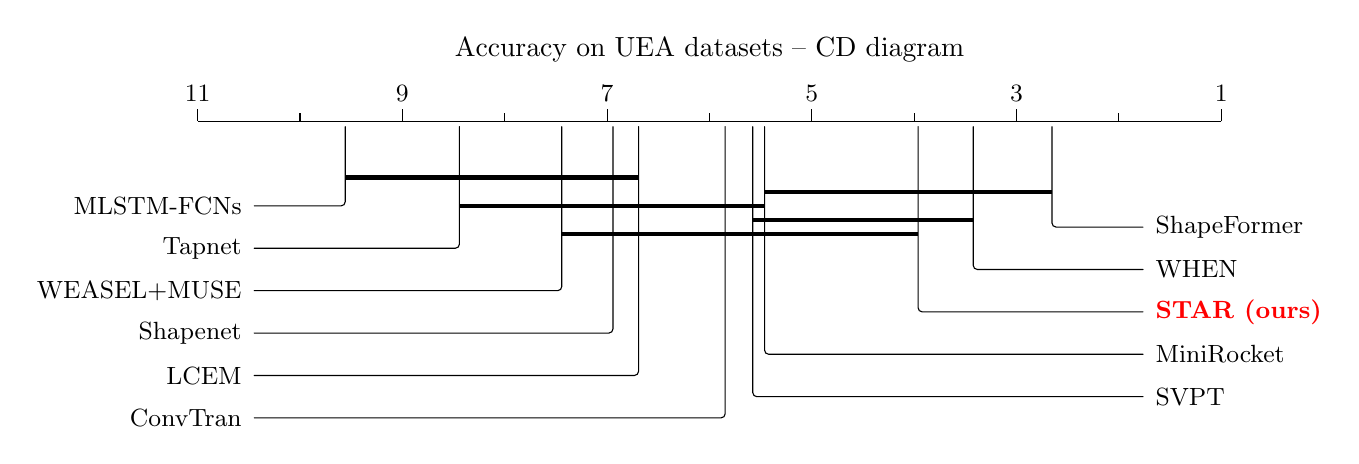
\begin{tikzpicture}[
  treatment line/.style={rounded corners=1.5pt, line cap=round, shorten >=1pt},
  treatment label/.style={font=\small},
  group line/.style={ultra thick},
]

\begin{axis}[
  clip={false},
  axis x line={center},
  axis y line={none},
  axis line style={-},
  xmin={1},
  ymax={0},
  scale only axis={true},
  width={13cm},
  ticklabel style={anchor=south, yshift=1.3*\pgfkeysvalueof{/pgfplots/major tick length}, font=\small},
  every tick/.style={draw=black},
  major tick style={yshift=.5*\pgfkeysvalueof{/pgfplots/major tick length}},
  minor tick style={yshift=.5*\pgfkeysvalueof{/pgfplots/minor tick length}},
  title style={yshift=\baselineskip},
  xmax={11},
  ymin={-6.5},
  height={3.5cm},
  xtick={1,3,5,7,9,11},
  minor x tick num={1},
  x dir={reverse},
  title={Accuracy on UEA datasets -- CD diagram},
]

\draw[treatment line] ([yshift=-2pt] axis cs:2.6538461538461537, 0) |- (axis cs:1.7371794871794872, -2.5)
  node[treatment label, anchor=west] {ShapeFormer};
\draw[treatment line] ([yshift=-2pt] axis cs:3.423076923076923, 0) |- (axis cs:1.7371794871794872, -3.5)
  node[treatment label, anchor=west] {WHEN};
\draw[treatment line] ([yshift=-2pt] axis cs:3.9615384615384617, 0) |- (axis cs:1.7371794871794872, -4.5)
  node[treatment label, anchor=west] {\textcolor{red}{\textbf{STAR (ours)}}};
\draw[treatment line] ([yshift=-2pt] axis cs:5.461538461538462, 0) |- (axis cs:1.7371794871794872, -5.5)
  node[treatment label, anchor=west] {MiniRocket};
\draw[treatment line] ([yshift=-2pt] axis cs:5.576923076923077, 0) |- (axis cs:1.7371794871794872, -6.5)
  node[treatment label, anchor=west] {SVPT};
\draw[treatment line] ([yshift=-2pt] axis cs:5.846153846153846, 0) |- (axis cs:10.474358974358974, -7.0)
  node[treatment label, anchor=east] {ConvTran};
\draw[treatment line] ([yshift=-2pt] axis cs:6.6923076923076925, 0) |- (axis cs:10.474358974358974, -6.0)
  node[treatment label, anchor=east] {LCEM};
\draw[treatment line] ([yshift=-2pt] axis cs:6.9423076923076925, 0) |- (axis cs:10.474358974358974, -5.0)
  node[treatment label, anchor=east] {Shapenet};
\draw[treatment line] ([yshift=-2pt] axis cs:7.4423076923076925, 0) |- (axis cs:10.474358974358974, -4.0)
  node[treatment label, anchor=east] {WEASEL+MUSE};
\draw[treatment line] ([yshift=-2pt] axis cs:8.442307692307692, 0) |- (axis cs:10.474358974358974, -3.0)
  node[treatment label, anchor=east] {Tapnet};
\draw[treatment line] ([yshift=-2pt] axis cs:9.557692307692308, 0) |- (axis cs:10.474358974358974, -2.0)
  node[treatment label, anchor=east] {MLSTM-FCNs};
\draw[group line] (axis cs:5.461538461538462, -2.0) -- (axis cs:8.442307692307692, -2.0);
\draw[group line] (axis cs:2.6538461538461537, -1.6666666666666667) -- (axis cs:5.461538461538462, -1.6666666666666667);
\draw[group line] (axis cs:3.9615384615384617, -2.6666666666666665) -- (axis cs:7.4423076923076925, -2.6666666666666665);
\draw[group line] (axis cs:6.6923076923076925, -1.3333333333333333) -- (axis cs:9.557692307692308, -1.3333333333333333);
\draw[group line] (axis cs:3.423076923076923, -2.3333333333333335) -- (axis cs:5.576923076923077, -2.3333333333333335);

\end{axis}
\end{tikzpicture}